% Copyright (c) 2022 Tobias Briones. All rights reserved.
% SPDX-License-Identifier: CC-BY-SA-4.0
%
% This source code is part of
% https://github.com/tobiasbriones/cp-unah-is911-microprocessors and is
% licensed under the Creative Commons Attribution Share Alike 4.0
% International License found in the LICENSE file in the root
% directory of this source tree or at https://spdx.org/licenses/CC-BY-SA-4.0

\documentclass[conference]{IEEEtran}
\usepackage{preamble}

\title{SOCKETS DE MICROPROCESADORES DE PC MODERNOS}
\author{
    
\includegraphics[width = 40mm]{images/logo-unah}\\[8ex]
    \IEEEauthorblockN{Tobias Briones}
    \IEEEauthorblockN{tobias.briones@unah.hn}
    \IEEEauthorblockA{\textit{Universidad Nacional Autónoma de Honduras} \\
    \textit{Ingeniería de Sistemas} \\
    \textit{I PAC 2022} \\
    \textit{IS911-MICROPROCESADORES}} \\\vspace*{20pt} \normalsize  \\
    \today
}

\begin{document}

    \maketitle

    \begin{abstract}
        En esta investigación se provee un resumen sobre los sockets para PC
        modernos año 2022.
    \end{abstract}

    \tableofcontents

    \import{}{footer}

    \section{Introducción}\label{sec:introduction}

    Los sockets son conectores que permiten la conectividad física y
    eléctrica del microprocesador a la tarjeta madre. Se le denominará a los
    sockets o slots como zócalos, ya que esa es su equivalencia en el español.

    \bigbreak

    Como se mencionó arriba, podemos afirmar sobre los zócalos el siguiente
    enunciado:

    \begin{displayquote}
        Un zócalo de CPU contiene uno o más componentes mecánicos que
        proporcionan conexiones mecánicas y eléctricas entre un
        microprocesador y una placa de circuito impreso (PCB). Esto permite
        colocar y reemplazar la unidad central de procesamiento (CPU) sin
        soldar.\\
        \small Fuente: Wikipedia $\mid$ CPU socket (traducido de inglés a
        español)~\cite{wikipedia-contributors-2022}
    \end{displayquote}

    \bigbreak

    Algunos tipos de sockets, por mencionar, tenemos~\cite{authortechnews-2020}: TR4, AM4, LGA 1151, 2066, sTRX4. Al momento
    de diseñar una configuración para un PC se debe tener en cuenta que la
    tarjeta madre sea compatible con el resto del hardware escogido y en
    particular, el socket sea el que corresponde al modelo del CPU que se
    deberá instalar.

    \subsection{Definición}\label{subsec:def}

    Una definición simple de un socket es:

    \begin{displayquote}
        El \textbf{socket/slot de CPU} o \textbf{zócalo de CPU} se refiere a
        un conector físico en la placa base de una computadora que acepta un
        solo chip físico. Muchas placas base pueden tener varios sockets que,
        a su vez, pueden aceptar chips de varios núcleos.\\
        \small Fuente: University Information Technology Services (traducido
        de inglés a español)~\cite{university-information-technology-services-2019}
    \end{displayquote}

    Los ordenadores personales (incluyendo PCs gaming) e industriales cuentan
    con sockets similares o iguales. Los sockets son mayormente encontrados
    en estos equipos a diferencia de dispositivos móviles como portátiles o
    teléfonos inteligentes los cuales traen el CPU soldado en la tarjeta
    madre o cuentan con un SoC (System on a Chip) el cual es un integrado que
    implementa el CPU, memoria y demás componentes en un solo chip.

    \begin{figure}[H]
        \centering
        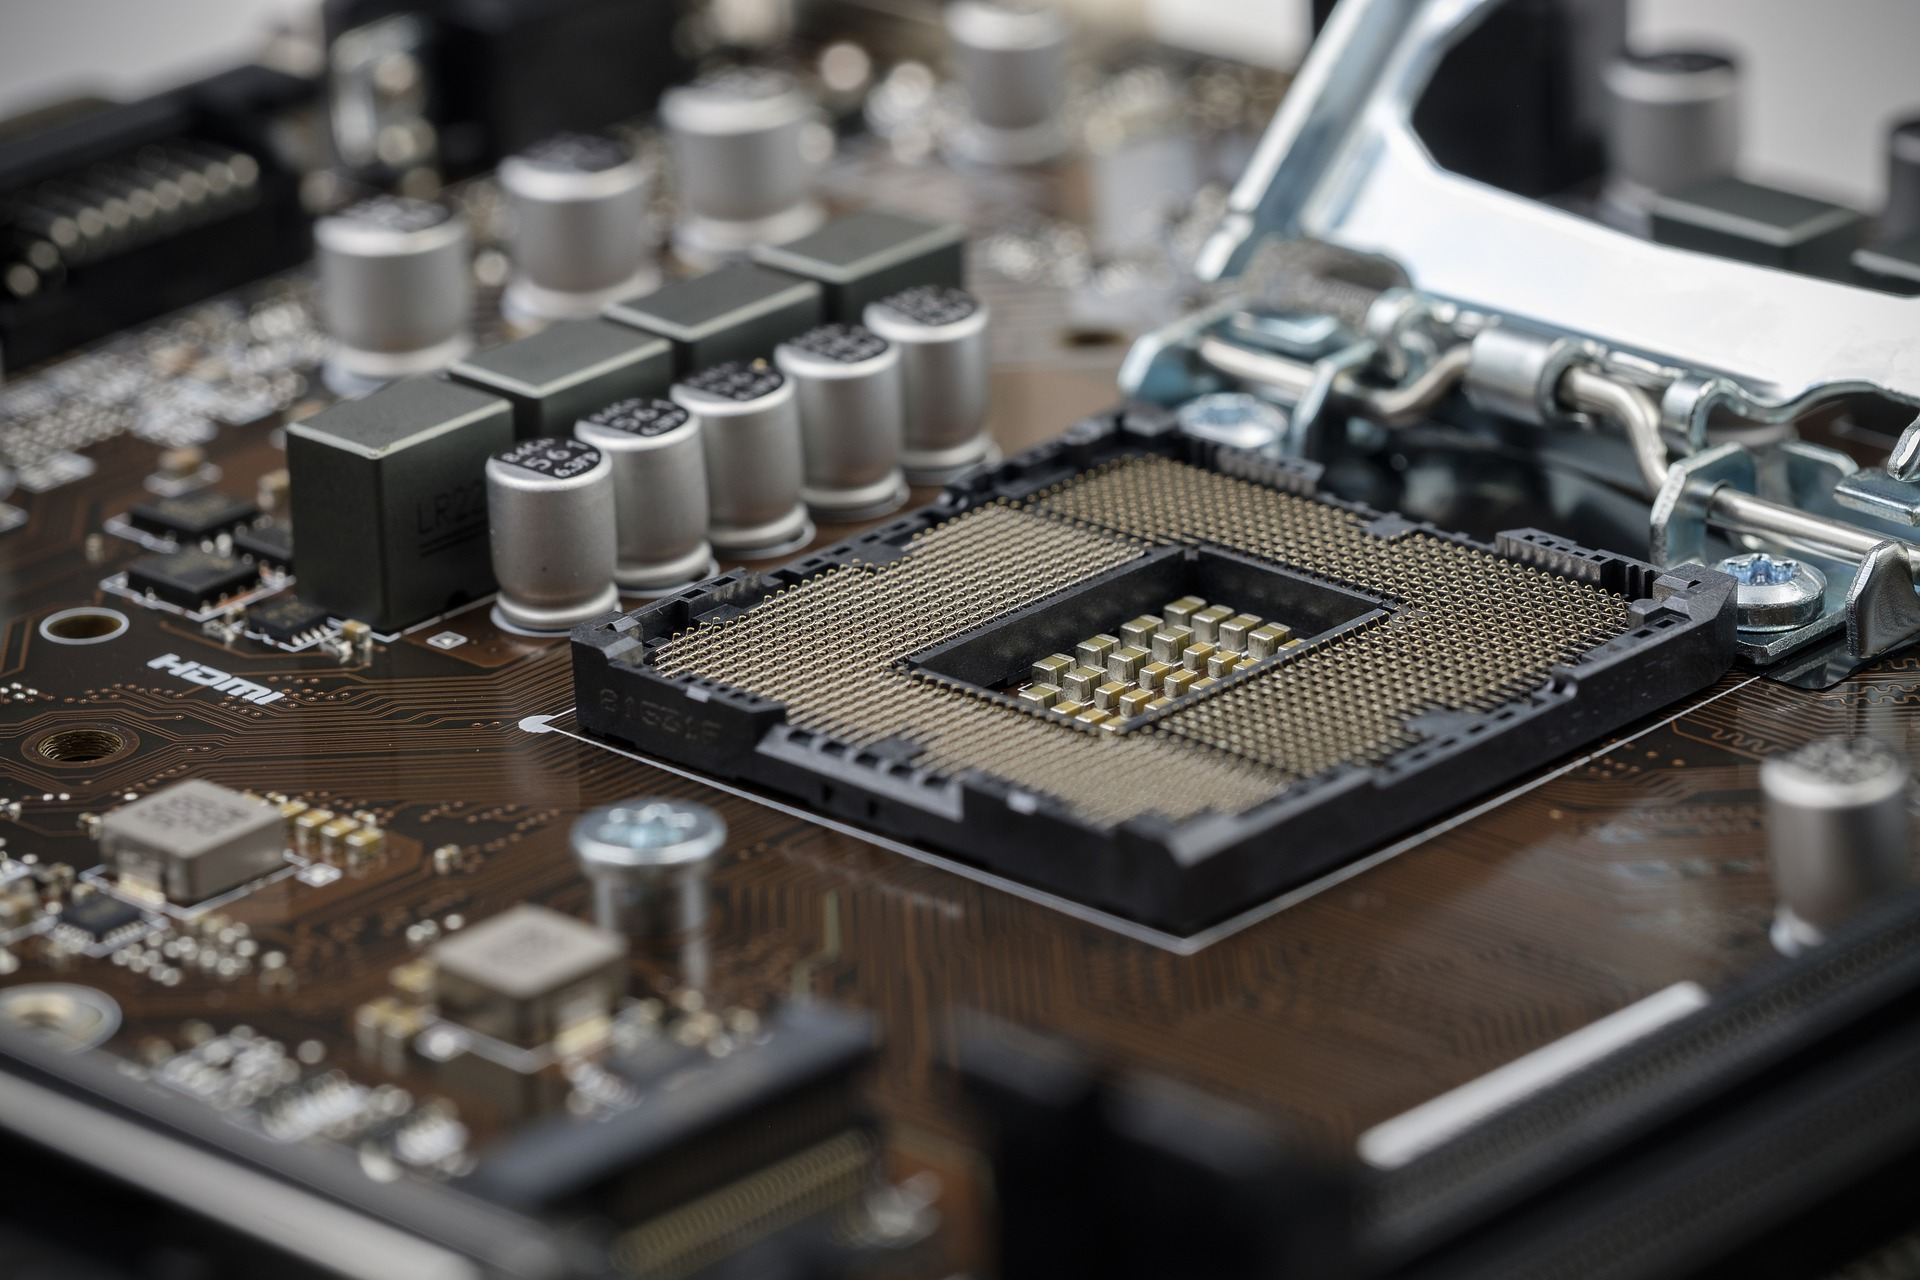
\includegraphics[width=0.3\paperwidth]{images/cpu-socket}
        \caption{Zócalo de CPU} \footnotesize
        Fuente: Imágen por \href{https://pixabay.com/users/bru-no-1161770}{Bruno /Germany} de \href{https://pixabay.com}{Pixabay}~\cite{pixabay-cpu-socket-2019}.\label{fig:figure}
    \end{figure}

    \section{Tipos de Zócalos}\label{sec:tipos-de-zócalos}

    De acuerdo a datos actuales, se van a presentar los tipos de zócalos que
    se utilizan en la actualidad para computadoras personales, gaming e
    incluso también workstation o industriales/servidores.

    \bigbreak

    Existe una gran cantidad de zócalos viejos \footnote{Wikipedia
    \cite{wikipedia-contributors-2022} enlista una gran cantidad de modelos
    incluyendo los viejos introducidos desde el año $1,970$. Si el lector es
    suficientemente viejo podrá reconocer algunos modelos como el $LGA 775$
        en el cual funcionaba nuestros viejos Intel Pentium 4/D o Core2Duo.},
    se detallarán solo los más recientes.

    \bigbreak

    Para escritorio PC se encuentran los siguientes modelos:

    \begin{table}[H]
        \centering
        \tiny
        \begin{tabular}{|l|l|l|l|l|}
            \hline
            \rowcolor[HTML]{CBCEFB}
            \textbf{\begin{tabular}[c]{@{}l@{}}
                        Nombre de \\ Zócalo
            \end{tabular}} & \textbf{\begin{tabular}[c]{@{}l@{}}
                                         Año de \\ Introducción
            \end{tabular}}   & \textbf{CPUs} & \textbf{Paquete} &
            \textbf{Pines} \\ \hline
            Socket AM5 & 2022 & AMD Zen 4 & LGA & 1718 \\ \hline
            \rowcolor[HTML]{EFEFEF}
            LGA 1700 & 2021 & Intel Alder Lake & LGA & 1700 \\ \hline
            LGA 1200 & 2020 & \begin{tabular}[c]{@{}l@{}}
                                  Intel Comet Lake\\ Intel Rocket Lake
            \end{tabular} & LGA & 1200 \\ \hline
            \rowcolor[HTML]{EFEFEF}
            \begin{tabular}[c]{@{}l@{}}
                Socket sTRX4/\\ Socket SP3r3
            \end{tabular} & 2019 & \begin{tabular}[c]{@{}l@{}}
                                       AMD Ryzen \\ Threadripper\\ (series 3,
                                       000)
            \end{tabular} & LGA & 4094 \\ \hline
            \begin{tabular}[c]{@{}l@{}}
                LGA 2066/Socket\\ R4
            \end{tabular} & 2017 & \begin{tabular}[c]{@{}l@{}}
                                       Intel Skylake-X\\ Intel Kaby Lake-X\\
                                       Intel Cascade Lake-X
            \end{tabular} & LGA & 2066 \\ \hline
            \rowcolor[HTML]{EFEFEF}
            \begin{tabular}[c]{@{}l@{}}
                Socket TR4/\\ Socket SP3r2
            \end{tabular} & 2017 & \begin{tabular}[c]{@{}l@{}}
                                       AMD Ryzen \\ Threadripper
            \end{tabular} & LGA & 4094 \\ \hline
            Socket AM4 & 2017 & \begin{tabular}[c]{@{}l@{}}
                                    AMD Ryzen 9\\ AMD Ryzen 7\\ AMD Ryzen 5\\
                                    AMD Ryzen 3\\ Athlon 200
            \end{tabular} & PGA & 1331 \\ \hline
        \end{tabular}
        \caption{Zócalos de CPU recientes}
        \small
        Fuente: Wikipedia \cite{wikipedia-contributors-2022}.
    \end{table}

    Los ordenadores se pueden clasificar en convencionales (PC o computador
    personal), HEDT (High-End Desktop son PC de alto rendimiento), o
    Servidores/Industriales/Estación de Trabajo. Los zócalos que se listaron
    son para PCs convencionales de escritorio con CPUs muy populares y
    algunos de alto rendimiento como los AMD Ryzen™ Threadripper™. Los Intel®
    Core™ X (LGA 2066/Socket R4) son un ejemplo de modelos para escritorio y
    para servidor también.

    \bigbreak

    Entre los modelos mencionados arriba y otros populares se resume la
    siguiente información más práctica que muestra el modelo de CPU(s),
    generación, chipsets compatibles y tipo de ordenador personal:

    \bigbreak

    \begin{itemize}
        \item \textbf{Intel LGA 2066:} 10ma Gen., X299, HEDT.
        \item \textbf{Intel LGA 1200:} 11/10ma Gen., Z490/H470, B460, H410,
        Convencional.
        \item \textbf{Intel LGA 1151:} 9/8va Gen.,
        Z390/Z370/Z370/Q370/H370/B365/B360/H310, Convencional.
        \item \textbf{AMD sTRX4:} Ryzen Threadripper 3000, TRX40, HEDT.
        \item \textbf{AMD TR4:} Ryzen Threadripper 2000 y 1000, x399, HEDT.
        \item \textbf{AMD AM4:} Ryzen 5000, 3000, 2000 y 1000,
        X570/X470/X370/B550/B450/B350/B450/A320/X300/A300, Convencional.
    \end{itemize}

    \small Fuente: tom'sHARDWARE~\cite{harding-2021}.

    \section{Funcionamiento}\label{sec:funcionamiento}

    De acuerdo al paquete del zócalo, se define su mecanismo de
    funcionamiento. Como se ha mencionado, el funcionamiento de un zócalo es
    tal que permite la conexión física del microprocesador a la tarjeta madre.

    \subsection{Matriz de Contactos en Rejilla (LGA)}\label{subsec:matriz-de
    -contactos-en-rejilla-(lga)}

    Los zócalos LGA son los más populares ya que como se ha visto
    anteriormente, muchos modelos de CPUs actuales para PCs normales lo
    utilizan.

    \bigbreak

    Según ONLOGIC Blog~\cite{fanton-2021} la mayoría de procesadores modernos
    removibles utilizan zócalo LGA.

    \bigbreak

    Su funcionamiento consiste en:

    \bigbreak

    \begin{displayquote}
        A diferencia de las interfaces de matriz de rejilla de pines (PGA) y
        matriz de rejilla de bolas (BGA), la interfaz LGA no presenta ni
        pines ni esferas, la conexión de la que dispone el chip es únicamente
        una matriz de superficies conductoras o contactos chapadas en oro que
        hacen contacto con la placa base a través del zócalo de CPU.

        \bigbreak

        Su alineación de pines es vertical y horizontal.

        \bigbreak

        Esta interfaz se beneficia por reducir el proceso de fabricación,
        amén de unas características térmicas, eléctricas y físicas
        superiores a las interfaces de chips previamente usados.\\
        \small
        Fuente: Wikipedia $\mid$ Land Grid Array (traducido de inglés a
        español)~\cite{wikipedia-lga-2021D}.
    \end{displayquote}

    \begin{figure}[H]
        \centering
        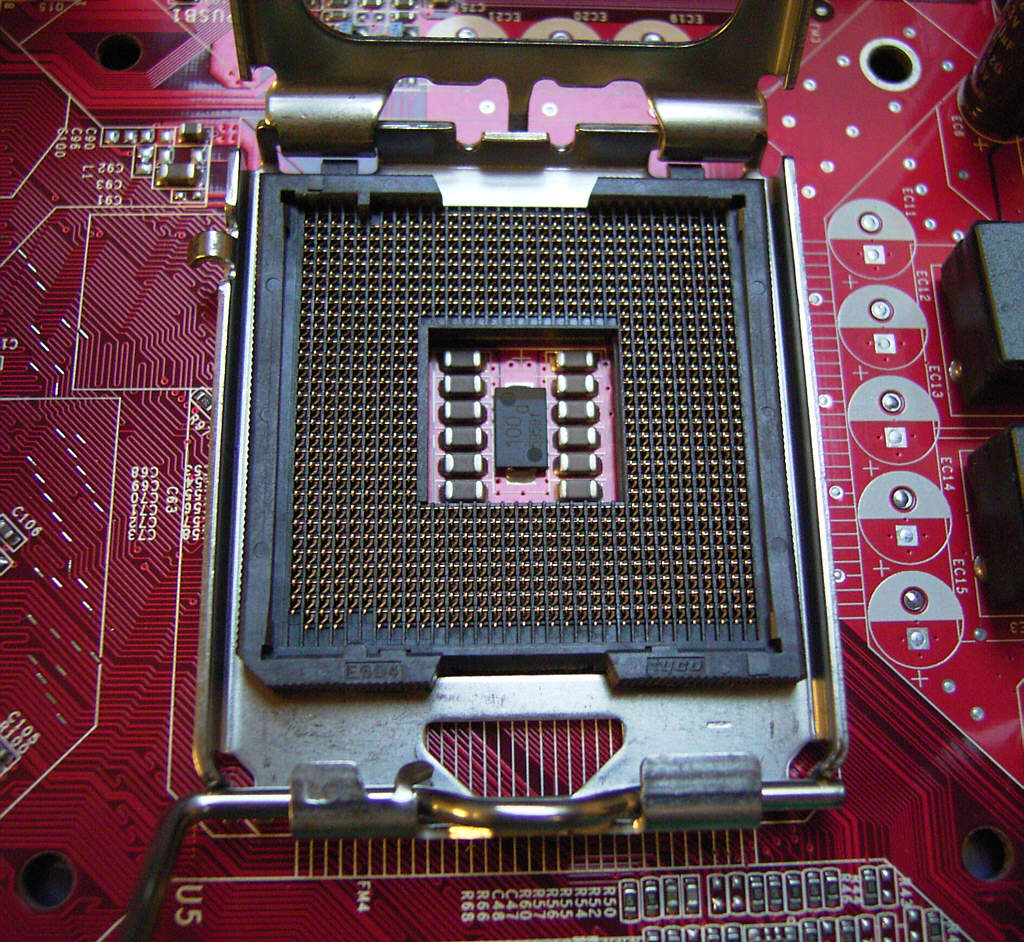
\includegraphics[width=0.2\paperwidth]{images/lga-socket}
        \caption{Zócalo de Matriz de Contactos en Rejilla} \footnotesize
        Fuente: De User Smial on de.wikipedia - Trabajo propio, CC BY-SA 2.0
        de, https://commons.wikimedia.org/w/index.php?curid=1066500
        \cite{wikipedia-lga-2021D}.\label{fig:figure2}
    \end{figure}

    \bigbreak

    Como se puede notar, ambos fabricantes mayores, AMD e Intel lo emplean
    para muchos de sus microprocesadores. Notar que, por ejemplo, el Socket
    sTRX4 es en realidad un LGA 4094~\cite{wikipedia-lga-2021D}.

    \subsection{Matriz de Rejilla de Pines (PGA)}\label{subsec:matriz-de
    -rejilla-de-pines-(pga)}

    Su funcionamiento consiste en:

    \bigbreak

    \begin{displayquote}
        En un PGA, el IC se monta en una losa de cerámica, que presenta una
        matriz de contactos o olas en una de sus caras. Luego, los pines se
        pueden insertar en los agujeros de un circuito impreso y soldarse.\\
        \small
        Fuente: Wikipedia $\mid$ Pin grid array (traducido de inglés a
        español)~\cite{wikipedia-pga-2021C}.
    \end{displayquote}

    \subsection{Matriz de Rejilla de Bolas (BGA)}\label{subsec:matriz-de
    -rejilla-de-bolas-(bga)}

    Estos son más que todo usados para móviles, portátiles o casos de uso en
    ingeniería eléctrica~\cite{wikipedia-bga-2021B} por lo que no nos
    interesan mucho en este artículo. Tenemos que:

    \begin{displayquote}
        Son usadas comúnmente en la producción y fijación de placas base para
        computadoras y la fijación de microprocesadores ya que los mismos
        suelen tener una cantidad muy grande de terminales los cuales son
        soldados a conciencia a la placa base para evitar la pérdida de
        frecuencias y aumentar la conductividad de los mismos.\\
        \small
        Fuente: Wikipedia $\mid$ Ball grid array (traducido de inglés a
        español)~\cite{wikipedia-bga-2021B}.
    \end{displayquote}

    \subsection{Cero Fuerza de Inserción (ZIF)}\label{subsec:cero-fuerza-de
    -inserción-(zif)}

    El zócalo ZIF (Zero Insertion Force) permite insertar el CI de forma muy
    fácil. Se ve por ejemplo, en los programadores de PIC donde el
    microcontrolador se inserta directamente en el socket.

    \begin{figure}[H]
        \centering
        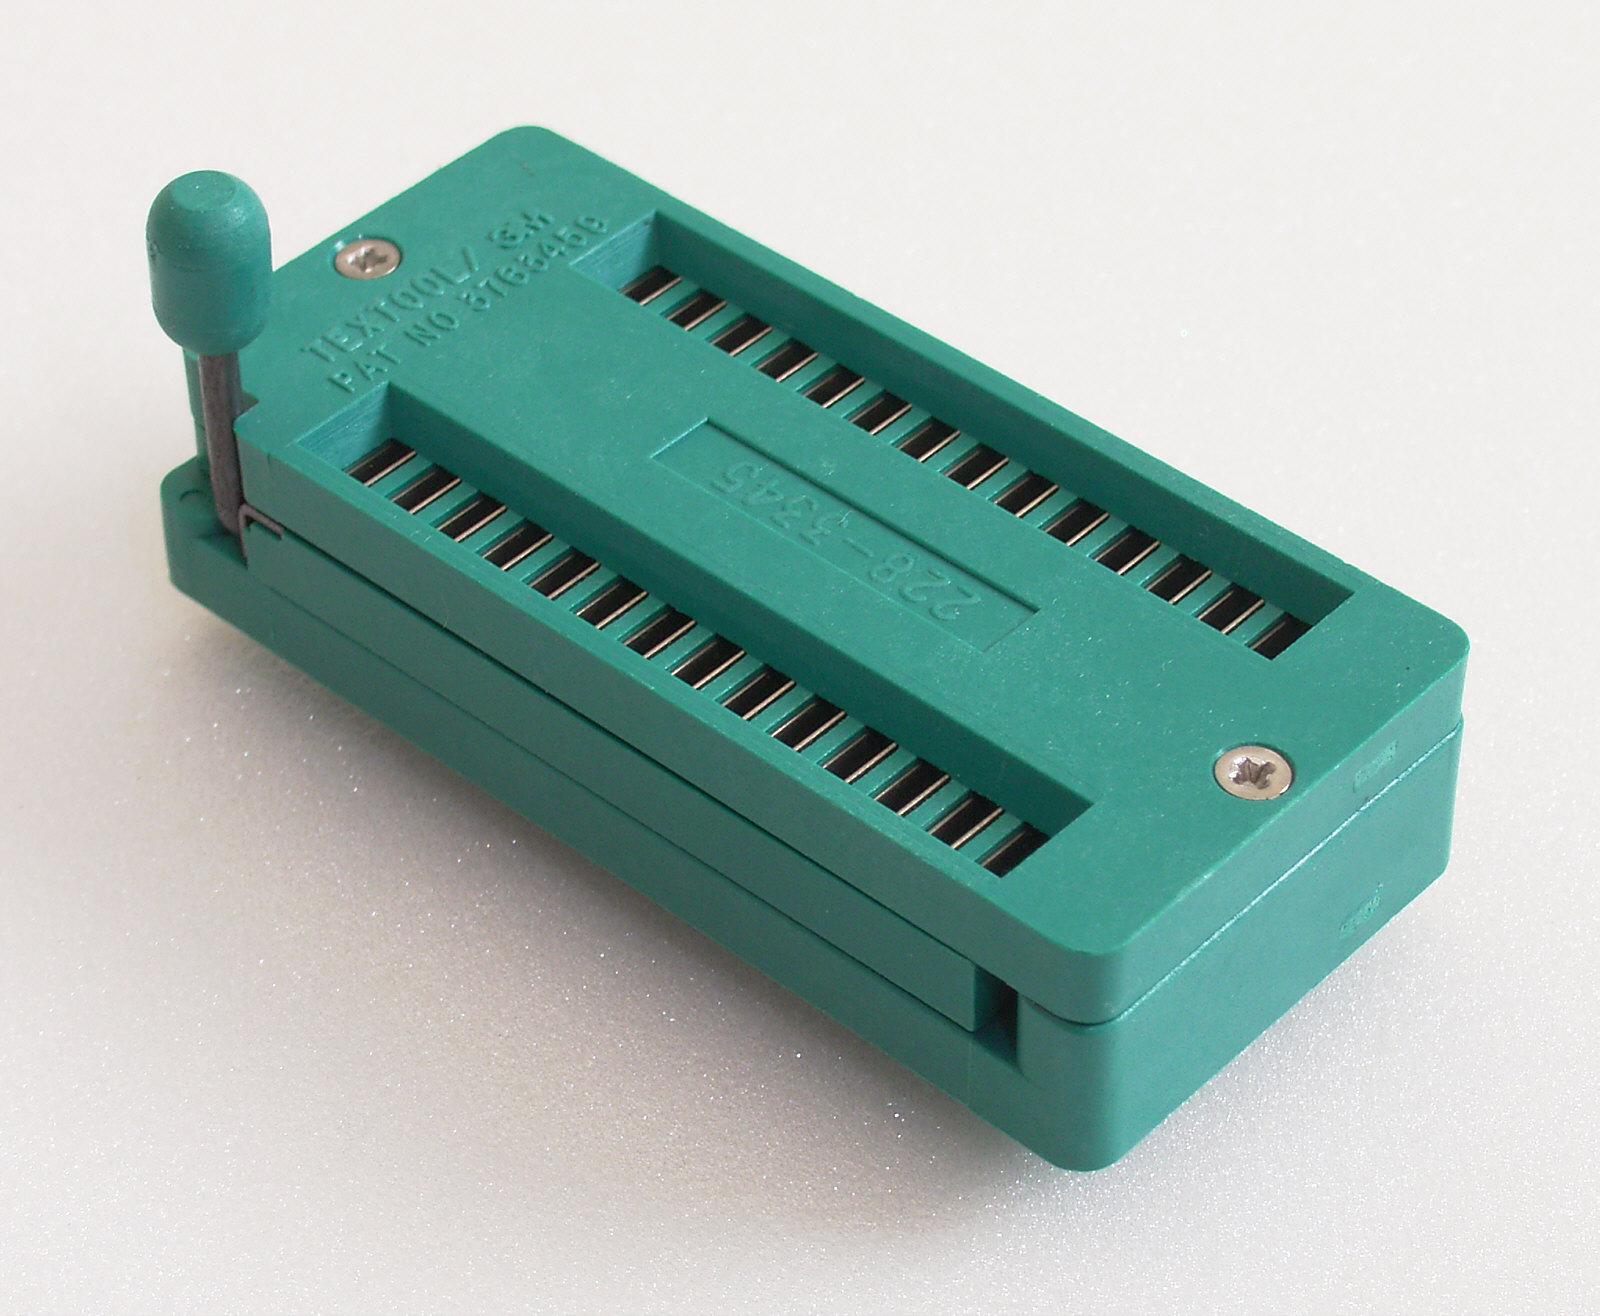
\includegraphics[width=0.2\paperwidth]{images/zif-socket}
        \caption{Zócalo de Cero Fuerza de Insersión} \footnotesize
        Fuente: Por usuario Smial en de.wikipedia - Trabajo propio, CC BY-SA
        2.0 de, https://commons.wikimedia.org/w/index.php?curid=1058788~\cite{wikipedia-zif-2021}.\label{fig:figure3}
    \end{figure}

    \bigbreak

    Su funcionamiento consiste en:

    \bigbreak

    \begin{displayquote}
        Fuerza de inserción cero (ZIF por sus siglas en inglés) es un tipo de
        zócalo para CI o conector eléctrico que requiere muy poca fuerza para
        la inserción. Con un zócalo ZIF, antes de insertar el CI, se mueve
        una palanca o deslizador en el costado del zócalo, separando todos
        los contactos suspendidos para que el CI pueda insertarse con muy
        poca fuerza; por lo general, el peso del CI en sí es suficiente y no
        se requiere ninguna fuerza externa hacia abajo. Luego, la palanca se
        mueve hacia atrás, lo que permite que los contactos se cierren y
        agarren los pines del CI. Los zócalos ZIF son mucho más caros que los
        zócalos de CI estándar y también tienden a ocupar un área de placa
        más grande debido al espacio que ocupa el mecanismo de palanca. Por
        lo general, solo se usan cuando hay una buena razón para hacerlo.\\
        \small
        Fuente: Wikipedia $\mid$ Zero Insertion Force (traducido de inglés a
        español)~\cite{wikipedia-zif-2021}.
    \end{displayquote}

    \bigbreak

    Por lo que también son zócalos de nicho y no nos interesa mucho por aquí.

    \section{Conclusión}\label{sec:conclusion}

    Se enlisto la información principal sobre los zócalos empleados en la
    actualidad año 2022 para microprocesadores convencionales o PCs. Se
    explicó brevemente como funcionan los zócalos de CPU y que hay categorías
    de PCs en función de las necesidades de los usuarios, las cuales
    requieren de distintos tipos de zócalos. Se observó que el paquete de
    zócalo LGA es el más utilizado para PCs.

    \printbibliography

\end{document}
